\documentclass{article}
\usepackage{geometry}
\geometry{margin=1in}
\usepackage{multirow}


%Figures
\usepackage{subcaption}
\usepackage{graphicx}
\usepackage{array}
\graphicspath{ {./images/} }

%Tables
\usepackage[table,xcdraw]{xcolor}
\usepackage{stfloats}
\usepackage{setspace}

\title{MAE 159 Midterm Aircraft Sizing Report}
\author{Thomas Slagle}
\date{May 7th, 2021}

\parskip=10pt

\begin{document}
    \maketitle

    \section{Introduction}
    \begin{flushleft}
        This report consists of a study on the cost and performance optimization
        for two subsoinc commercial transport aircraft, one non-stop aircraft
        and one one-stop aircraft. Herein, the reader will find a summary of the
        methods used and the data generated from an itterative python script
        which uses standard, well-defined aircraft deisgn methods to exactly
        meet the design specifications. Various parameters, including ... , were
        systematically varied to determine the optimum design parameters. In the
        conclusion of the report, the optimum design parameters will be given as
        well as an summary of why the design was chosen, and how the which of
        the two optimized aircraft may suit the customer's needs the best.
    \end{flushleft}

    \section{Design Specifications}
    \begin{flushleft}
        As mentioned prior, two aircraft with distinct given design
        requirements, were considered in this design study. Both aircraft are
        requried to carry 225 passangers adn complete a 7400 nautical mile
        journey. The first larger aircraft must compelte the journey without any
        stops. The second smaller aircraft must complete the journey with
        one-stop, giving the airplane a required range of 3700 nautical miles.
        The complete set of given design specifications are listed in tables 1
        and 2 below. For both aircraft, takeoff conditions were assumed to be at
        sea level on a hot day with an air temperature of $84^{\circ}F$.
    \end{flushleft}

    \begin{table}[ht]
    \begin{tabular}{|c|c|}
    \hline
    \rowcolor[HTML]{FFC702}
    \multicolumn{2}{|c|}{\cellcolor[HTML]{FFC702}\textbf{Non-stop Aircraft}} \\ \hline
    \textbf{Design Specification:}        & \textbf{Parameter Value:}        \\ \hline
    Number of Passangers                  & 225                              \\ \hline
    \rowcolor[HTML]{C0C0C0}
    Weight of Cargo                       & 6,000 lbs                        \\ \hline
    Still Air Range                       & 7,400 nmi                        \\ \hline
    \rowcolor[HTML]{C0C0C0}
    Takeoff Field Length                  & 10,500 ft                        \\ \hline
    Landing Approach Speed                & 140 kts                          \\ \hline
    \rowcolor[HTML]{C0C0C0}
    Fuel Destination Payload              & 35\%                             \\ \hline
    Cruise Mach Number                    & 0.85                             \\ \hline
    \rowcolor[HTML]{C0C0C0}
    Initial Cruise Altitude               & 35,000 ft                        \\ \hline
    \end{tabular}
    \quad
    \begin{tabular}{|c|c|}
        \hline
        \rowcolor[HTML]{DAE8FC}
        \multicolumn{2}{|c|}{\cellcolor[HTML]{DAE8FC}\textbf{One-stop Aircraft}} \\ \hline
        \textbf{Design Specification:}        & \textbf{Parameter Value:}        \\ \hline
        Number of Passangers                  & 225                              \\ \hline
        \rowcolor[HTML]{C0C0C0}
        Weight of Cargo                       & 3,000 lbs                        \\ \hline
        Still Air Range                       & 3,700 nmi                        \\ \hline
        \rowcolor[HTML]{C0C0C0}
        Takeoff Field Length                  & 6,000 ft                         \\ \hline
        Landing Approach Speed                & 130 kts                          \\ \hline
        \rowcolor[HTML]{C0C0C0}
        Fuel Destination Payload              & 0\%                              \\ \hline
        Cruise Mach Number                    & 0.80                             \\ \hline
        \rowcolor[HTML]{C0C0C0}
        Initial Cruise Altitude               & 35,000 ft                        \\ \hline
    \end{tabular}
    \end{table}

\section{Design Analysis}
    \begin{flushleft}
        The object of this section is to perform an analysis for both aircraft
        and determine the optimized specifications for the design parameters
        such as aspect ratio, number of aisles, number of engines, number of
        seats abreast, and more. An itterative python script was written with
        allowable user input for user-selectable design parameters to make
        calculations of direct operating cost (DOC), weight, drag, and other
        airfact performance charactersitics easy, fast, and repeatable.
    \end{flushleft}

    \subsection{Aspect Ratio Variation}
        \begin{flushleft}
            The aspect ratio describes the ratio of the airfact's wingspan to
            its mean aerodynamic chord length. A small aspect ratio describes a
            short and wide wing whereas a larger aspect ratio describes a long
            and narrow wing planform. The wing aspect ratio is an important
            factor in determing the available lift of the aircraft, the weight
            of the aircraft, and the induced drag during flight. For a typical
            jet transport aircraft, Schaufele gives an aspect ratio range of 7.0
            to 9.5, as such, this formed the basis for design selection. Aspect
            ratios in steps of 0.5 were considered from 6.0 to 10.0 during this
            study. The method for comparison will be the resulting DOC per
            passanger, per mile. Figure \ref{fig:doctmAR} shows sweep angle versus
            the DOC with curves of fixed aspect ratio for both aircraft.
            \begin{figure*}[ht]
                \centering
                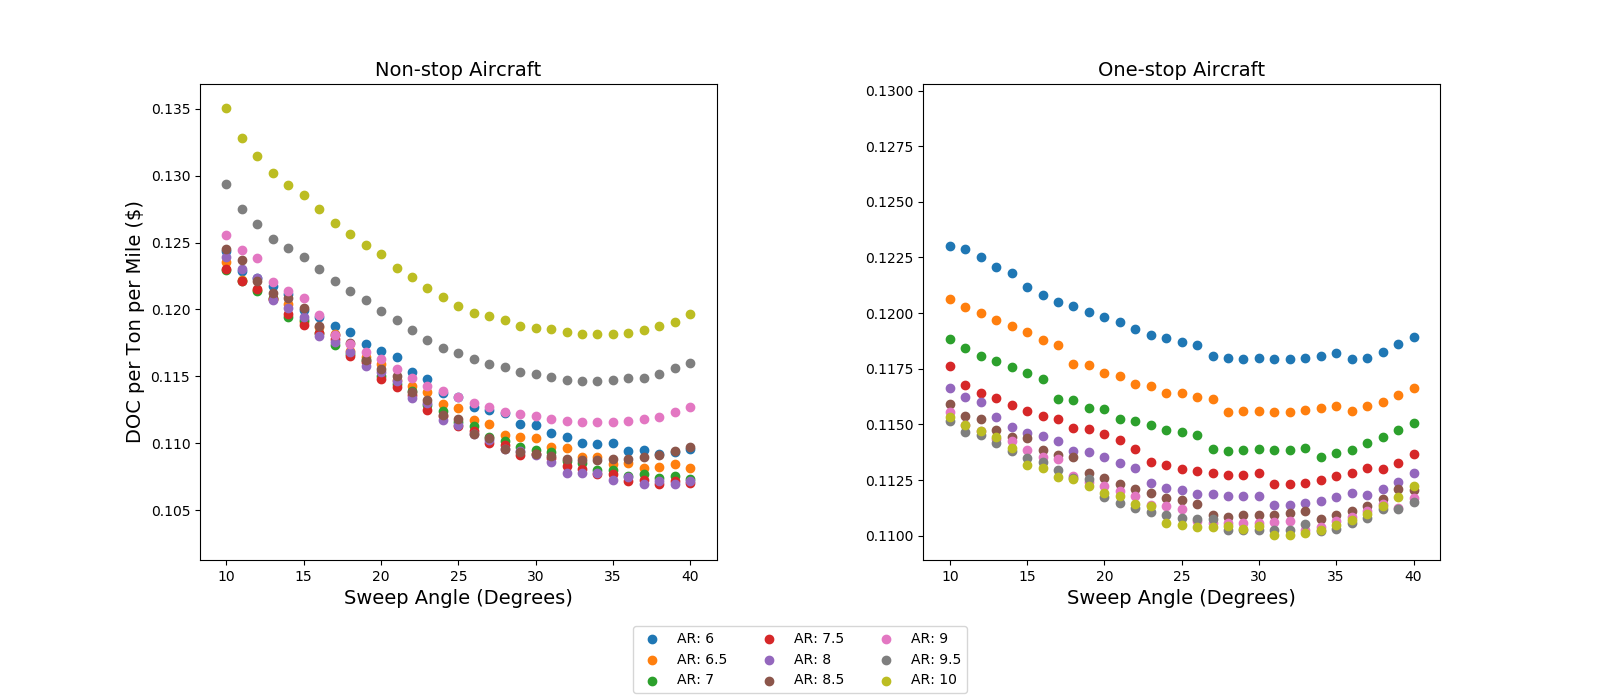
\includegraphics[scale=0.4]{DOCTM v Sweep Angle.PNG}
                \caption{Direct operating cost, per ton, per mile plotted against sweep angle for the non-stop and one-stop aircraft at different aspect ratios.}
                \label{fig:doctmAR}
            \end{figure*}

            From figure \ref{fig:doctmAR}, it is evident that for the non-stop
            aircraft, the optimized aspect ratio is between 7.5 and 8. For the
            one-stop aircraft, the optimized aspect ratio is between 9.5 and 10.
        \end{flushleft}
    \subsection{Wing Sweep Angle Variation}
        \begin{flushleft}
            Starting with the best two values of aspect ratio determine from the
            aspect ratio variation plots, the optimized wing sweep angle can be
            determined by plotting the DOC against the wing sweep angle. For
            easier interpertation of the data, only the best two aspect ratios
            obtained in the previous subsection were utilized in this
            determination. These results are plotted in figure \ref{fig:AR}.

            \begin{figure*}[ht]
                \centering
                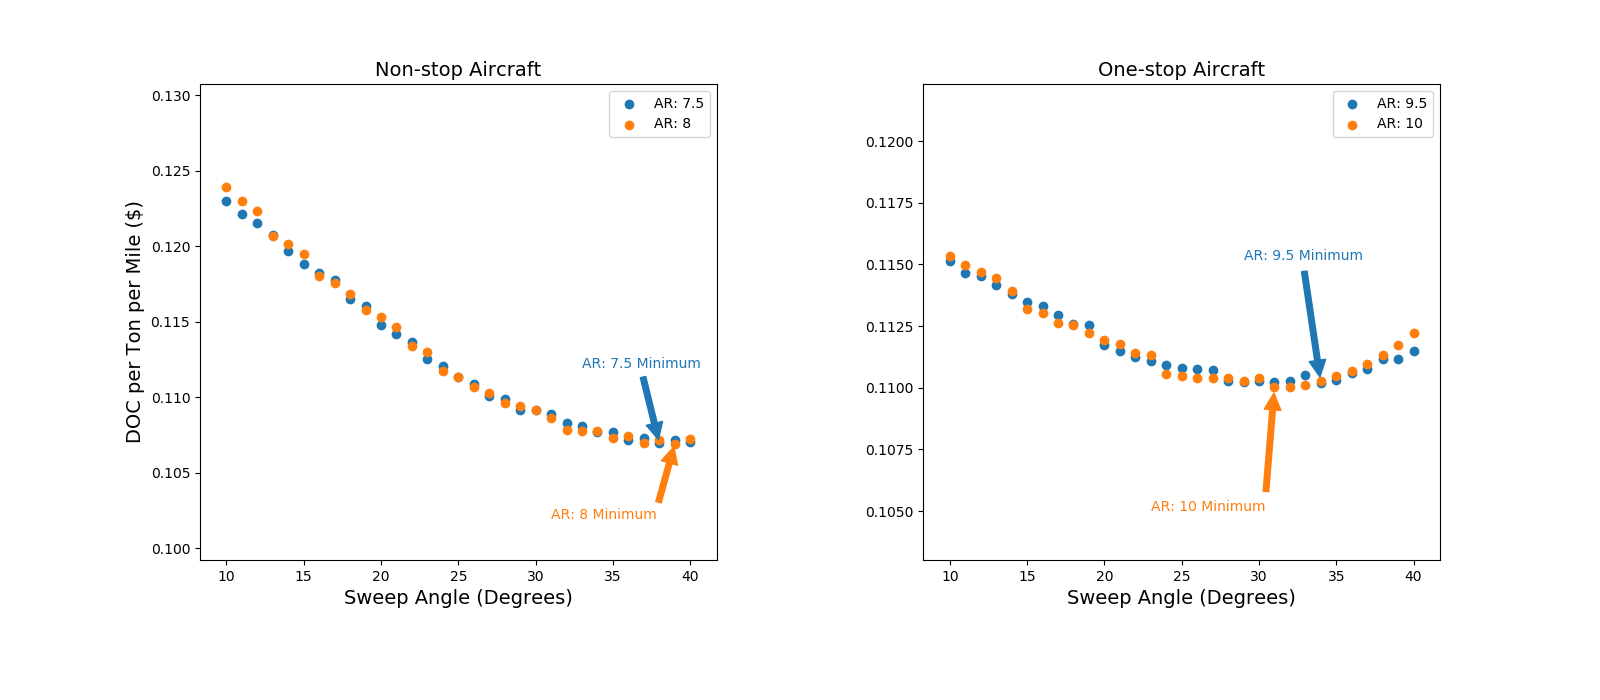
\includegraphics[scale=0.4]{AR Plot.PNG}
                \caption{Direct operating cost, per ton, per mile plotted against sweep angle for the non-stop and one-stop aircraft at the optimized aspect ratios.}
                \label{fig:AR}
            \end{figure*}

            From figure \ref{fig:AR}, it is determined that the minimum DOC per
            ton, per mile is \$0.1069204 and \$0.11001131 for the non-stop and
            one-stop aircraft respectively. These lowest DOC values correspond
            to an asepct ratio of 8 with a sweep angle of 39 degrees for the
            non-stop aircraft and an aspect ratio of 10 with a sweep angle of 31
            degrees. Interestingly, in this configuration, the optimized
            non-stop aircraft has a lower DOC than the optimized one-stop
            aircraft.

        \end{flushleft}

    \subsection{Advanced Technology (aluminum v composite, conventional v supercritical)}
        \begin{flushleft}
            Modern technology and manufacturing advancements has allowed for the
            use of more exotic airfoil shapes that previous heritage aircraft
            could not take advantage of. Supercritical airfoils have been cited
            to improve aircraft fuel efficiency and thus lower the direct
            operating cost of the aircraft. The Boeing 757 and 767, developed
            during the 1980s were some of the first commerical aircraft to use
            this technology. However, these airfoils types are comprised of more
            complciated compund curves which presents added complexity in the
            manufacturing process, driving up initial cost of the aircraft
            however, the decrease in operational costs of the aircraft exceeds
            the initial procurement cost increase of the aircraft. Figure
            \ref{fig:supercritical} plots the direct operating cost of the
            aircraft versus the sweep angle for the optimized aspect ratios
            obtained in the previous sections, and with the implementation of
            the supercritical airfoil versus the wing sweep angle. It is evident
            that for all vlaues of the sweep, the DOC was lower when
            implementing the supercritical airfoil technology to the aircrafts'
            wings. However, the optimal sweep angle shifted for both aircraft
            when the aspect ratio was held constant, from the optimized value
            gathered from the previous section, section 3.1.

            \begin{figure*}[ht]
                \centering
                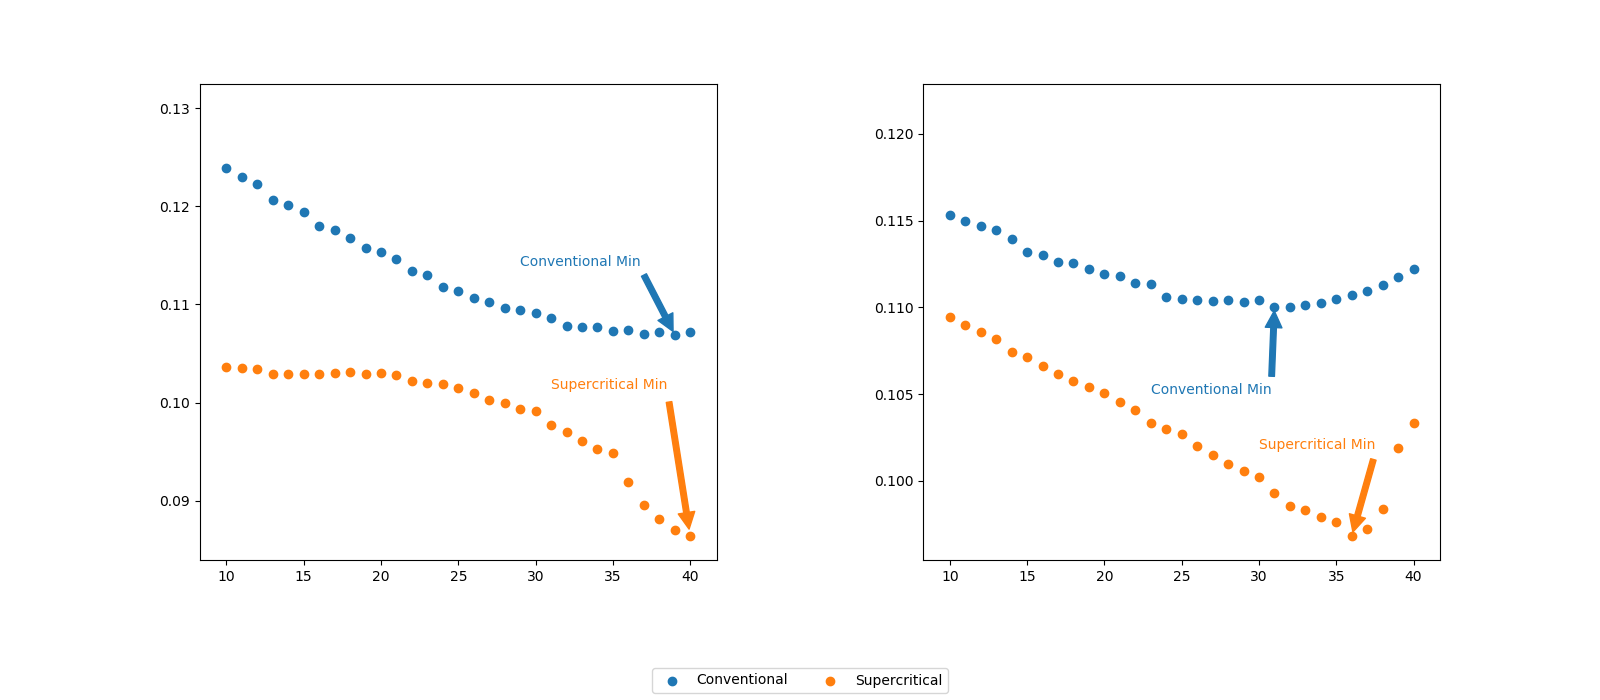
\includegraphics[scale=0.4]{CvS.PNG}
                \caption{Direct operating cost, per ton, per mile plotted against sweep angle for the non-stop and one-stop aircraft at the optimized aspect ratios, while comparing the effects of a supercritcal wing airfoil.}
                \label{fig:supercritical}
            \end{figure*}

            Using the supercritical airfoil technology with an aspect ratio of 8
            and 10 for the nonstop and onstop aircraft respectively, the minimum
            direct operating cost per ton, per mile were \$0.08639182 and
            \$0.09680141, with wing sweep values of 40 degrees and 36 degrees,
            for the nonstop and onstop aircraft respectively. Again, the nonstop
            aircraft had a lower direct operating cost than the onestop
            aircraft.

        \end{flushleft}

    \subsection{Aircraft Seat Configuration}
        \begin{flushleft}
            The aircraft seat configuration can also be varied. In this case,
            the main metric of comparison will be the direct operating cost.
            Both the supercritical and conventional airfoil types were
            considered in this section of the study as well. It stands to reason
            that the supercritical airfoil will be the optimal choice regardless
            of the seat configuration however for sake of robustness. Above, the
            standard configuration of two aisles and eight passangers abreast
            were considered. However, there are other options for seat layout of
            the passanger seating area. For sake of brevity, only one other
            common seating layout was considered, the single aisle, six
            passangers abreast configration. These results are plotted in figure \ref{fig:seats}

            \begin{figure*}[ht]
                \centering
                \includegraphics[scale=0.4]{}
                \caption{Direct operating cost, per ton, per mile plotted against sweep angle for the non-stop and one-stop aircraft at the optimized aspect ratios. Both the conventional and supercritical airfoil types were considered in this analysis. The number of seats and aisles were varied.}
                \label{fig:seats}
            \end{figure*}

            From this study, it is evident that the optimal sweep angle did not
            change for either the supercritical or convnetional airfoil
            configuration, when the seating configuration was changed. However,
            it is clear

        \end{flushleft}


\end{document}
